% SPDX-FileCopyrightText: © 2026 Idiap Research Institute <contact@idiap.ch>
%
% SPDX-FileContributor: Andre Freitas <andre.freitas@idiap.ch>
% Neuro-symbolic AI Group
%
% SPDX-FileContributor: Danilo Gusicuma <danilo.gusicuma@idiap.ch>
% Neuro-symbolic AI Group
%
% SPDX-License-Identifier: MIT
\section{From a candidate explanation to a scoped conclusion}
Consider diffusion on a network. A researcher wants to know when local exchange produces rapid equilibration across networks of increasing size. We use four reasoning mechanisms to separate proposing an explanation, deriving its consequences, challenging its scope, and deciding what remains justified. These mechanisms make distinct inferential responsibilities visible within the candidate-to-status motif. They are not an exhaustive account of inquiry: induction, structural transfer, modeling, and contrast supply other essential transformations.

\paragraph{Abduction proposes what could explain the gap.}
Given a question and relevant constraints, abduction produces a candidate premise or mechanism. It expands the possibilities without establishing any of them. For diffusion, the researcher proposes that a lower bound on the network's spectral gap could explain rapid relaxation. The candidate is scientifically useful because it identifies a specific missing condition to investigate. Merely saying that a network is connected does not yet supply that bound. Abduction therefore contributes a possible explanation and an obligation, rather than an entailed conclusion.

\paragraph{Deduction exposes what follows if the premises hold.}
Deduction consumes explicit premises and produces a consequence that retains their scope. Let $L$ be the symmetric Laplacian of a finite connected graph, with unit edge rates, and let a mean-zero deviation $u$ obey $\dot u=-Lu$. If its first nonzero eigenvalue satisfies $\lambda_1(L)\geq c>0$, orthogonal eigenmode decomposition gives
\[
  \|u(t)\|_2\leq e^{-ct}\|u(0)\|_2,\qquad t\geq0.
\]
This explains why a spectral bound would control relaxation. It does not establish the proposed bound for the researcher's network family. The premise can become the next proof obligation; it cannot disappear when the consequence is passed downstream.

\paragraph{Refutation searches for where the claim breaks.}
Refutational reasoning consumes a claim or route together with a critical test, and returns a supported defeater or a bounded test outcome. To challenge a size-independent relaxation claim from connectedness alone, take the unweighted cycle $C_n$, $n\geq3$. Its spectral gap is
\[
 \lambda_1(C_n)=2-2\cos(2\pi/n)\longrightarrow0.
\]
Every member is finite and connected, yet no positive gap lower bound holds across the entire family. For example, the gaps at $n=4$ and $n=16$ are $2$ and approximately $0.1522$: the slowest relaxation becomes over thirteen times slower. Initial data in the slow eigenmode defeats the proposed uniform rate. The counterexample attacks the missing uniformity premise, not the conditional eigenmode deduction. Failure to find such a counterexample would, by itself, establish neither that premise nor the original claim.

\paragraph{Calibration states exactly what survived.}
Calibration consumes the conditional result and the critical evidence, then assigns a justified status. Here the result is: exponential decay for each fixed graph, a uniform bound conditional on a separately established uniform spectral gap, and rejection of connectedness alone as a sufficient family-wide condition. The useful outcome is a sharper research question: which additional network conditions provide that uniform gap? Calibration introduces no new spectral estimate and supplies no missing proof. It changes what the existing result licenses and which obligation should be investigated next.

\section{Composition carries the burden forward}
The mechanism is not the mere list ``abduce, deduce, refute, calibrate.'' Its force comes from the relations between outputs and inputs:
\begin{figure}[htbp]
\centering
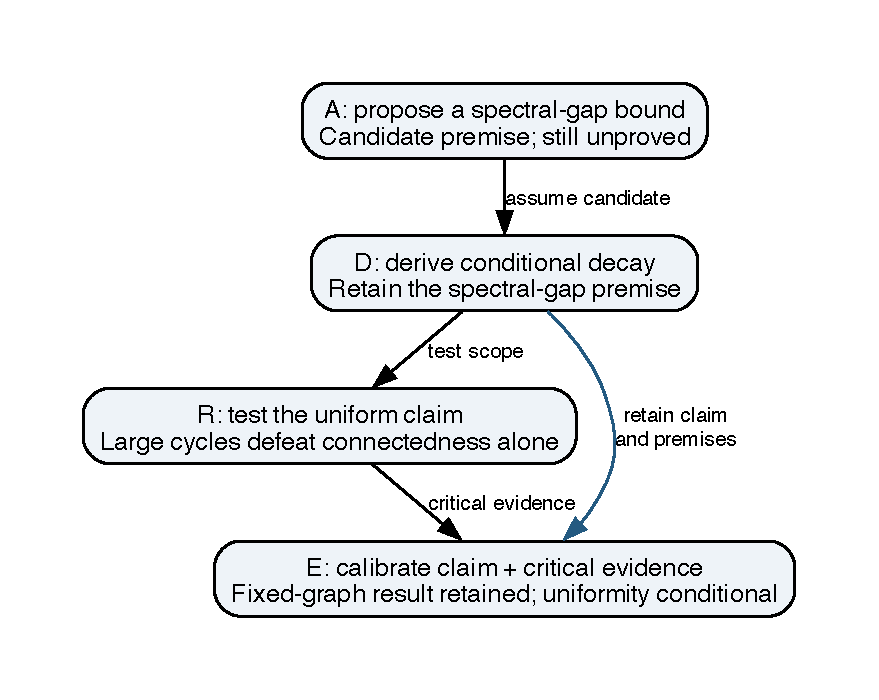
\includegraphics[width=.82\linewidth,height=.42\textheight,keepaspectratio]{paper-workflow-representations/core-workflow.pdf}
\caption{A constructed diffusion example makes the core inferential moves visible. Calibration receives both the retained conditional claim and the critical evidence. Arrows express information dependencies in the full conceptual motif, not a universal execution policy.}
\label{fig:core-workflow}
\end{figure}
The assumption relation authorizes reasoning under an assumption; it does not verify it. The testing relation exposes the consequence to a test that can distinguish fixed-size decay from uniform decay. The diagram makes the retained dependency explicit: calibration receives both the conditional decay claim, with its premises, and the uniformity defeater. It revises their justified scope together rather than replacing the claim with a verdict alone. Changing the test to ``the graph is connected'' would lose precisely the distinction the research problem needs.

This cycle is a \emph{motif}: an arrangement of mechanisms, not a ninth primitive operator. In the native local-work flow, an abductive route is assumed by deduction, its claim is tested by refutation, and claim plus verdict feed calibration. The source also declares an early stop on refutation; the conceptual chain above describes the full main path and does not assert that every executable branch reaches calibration.

Two contrasts explain why composition matters. A proof-delivery motif starts with supplied premises and uses deduction, refutation, and calibration; inventing an attractive hypothesis would not discharge an exact proof obligation. A plural-discovery motif combines a candidate with an induced pattern, then exposes both to model-based and contrastive probes before testing and calibration. In the diffusion example, apparent fast decay in a few small networks could motivate a conjecture; comparing increasingly large cycles with a family for which a gap bound is established would probe its uniformity. This is an illustrative use of that motif, not reported experimental evidence. Branches contribute different burdens rather than multiple votes for the same claim.

The typed account that follows formalizes these already visible distinctions: which kind of result can be consumed, under which license, and with which unresolved premises. Exhaustive workflow inventories and detailed formal reconstructions belong in the appendix; the central argument is the change in epistemic responsibility at each transition.

\paragraph{Evidence boundary.}
The native descriptions support this account of the intended operations. They do not, by themselves, establish execution reliability or improved scientific performance.

The concrete nominal interfaces and their successful-result adapters appear in Appendix~\ref{app:native-workflow}; Appendix~\ref{app:dependent-workflow} develops a claim-indexed presentation of the same retained dependency. Appendix~\ref{app:reasoning-taxonomy} locates the eight reasoning types within the functional taxonomy.
